\documentclass[10pt,a4paper]{article}

% --- PACKAGES ---
\usepackage[utf8]{inputenc}
\usepackage[T1]{fontenc}
\usepackage{helvet}
\renewcommand{\familydefault}{\sfdefault}
\usepackage{microtype}
\usepackage[margin=10mm,top=10mm,bottom=10mm]{geometry}
\usepackage[table]{xcolor}
\usepackage{graphicx}
\usepackage{amsmath,amssymb}
\usepackage{tabularx}
\usepackage{booktabs}
\usepackage{array}
\usepackage{enumitem}
\usepackage{fontawesome5}
\usepackage{tikz}
\usetikzlibrary{positioning,calc,shapes.geometric,arrows.meta,backgrounds}
\usepackage[most]{tcolorbox}
\usepackage{hyperref}

% --- COLOR PALETTE ---
\definecolor{Primary}{HTML}{0F172A}    % Slate 900
\definecolor{Accent}{HTML}{0EA5E9}     % Sky 600
\definecolor{AccentDark}{HTML}{0284C7} % Sky 700
\definecolor{BgLight}{HTML}{F8FAFC}    % Slate 50
\definecolor{CardBg}{HTML}{F1F5F9}     % Slate 100
\definecolor{LineColor}{HTML}{CBD5E1}  % Slate 300
\definecolor{TextDark}{HTML}{1E293B}   % Slate 800
\definecolor{TextMuted}{HTML}{64748B}  % Slate 500

\hypersetup{
    colorlinks=true,
    linkcolor=Accent,
    urlcolor=Accent,
    pdftitle={Synapse Core-X9 Enterprise AI Accelerator Datasheet},
    pdfauthor={Synapse Technologies Inc.}
}

\pagestyle{empty}
\setlength{\parindent}{0pt}
\setlength{\parskip}{0pt}

% --- CUSTOM STYLES ---
\tcbset{
    boxrule=0.6pt,
    arc=3pt,
    left=6pt,
    right=6pt,
    top=6pt,
    bottom=6pt,
    colframe=LineColor,
    colback=white
}

\newcommand{\sectionheading}[2]{%
  \vspace{2pt}%
  \begin{tcolorbox}[
    colback=Primary,
    colframe=Primary,
    arc=2pt,
    left=6pt,right=6pt,top=4pt,bottom=4pt,
    boxrule=0pt
  ]
    \textcolor{white}{\small\bfseries\makebox[1.2em][l]{#1} \MakeUppercase{#2}}
  \end{tcolorbox}%
  \vspace{4pt}%
}

\begin{document}

% ==================== HEADER BANNER ====================
\begin{tcolorbox}[
  colback=Primary,
  colframe=Primary,
  arc=4pt,
  left=10pt,right=10pt,top=10pt,bottom=10pt,
  boxrule=0pt
]
  \begin{minipage}[c]{0.70\textwidth}
    \textcolor{Accent}{\bfseries\scriptsize SYNAPSE TECHNOLOGIES \textbullet{} HARDWARE DATASHEET}\\[2pt]
    \textcolor{white}{\Huge\bfseries Synapse Core-X9}\\[2pt]
    \textcolor{Accent!30}{\large\bfseries Enterprise AI Acceleration Engine}\\[4pt]
    \textcolor{white}{\small High-performance PCIe Gen 5.0 inference engine for real-time edge intelligence and deep learning workloads.}
  \end{minipage}%
  \hfill
  \begin{minipage}[c]{0.26\textwidth}
    \begin{tcolorbox}[
      colback=Primary!80!black,
      colframe=Accent,
      boxrule=0.8pt,
      arc=3pt,
      left=4pt,right=4pt,top=6pt,bottom=6pt,
      halign=center
    ]
      \textcolor{white}{\scriptsize\bfseries STATUS: PRODUCTION}\\[2pt]
      \textcolor{Accent}{\small\bfseries REV Q3-2026}\\[2pt]
      \textcolor{white}{\tiny PART: SYN-X9-64G}
    \end{tcolorbox}
  \end{minipage}
\end{tcolorbox}

\vspace{6pt}

% ==================== METRIC HIGHLIGHT CARDS ====================
\begin{minipage}[t]{0.235\textwidth}
  \begin{tcolorbox}[colback=BgLight,colframe=LineColor,halign=center,top=5pt,bottom=5pt]
    \textcolor{AccentDark}{\faMicrochip\ \large\bfseries 750 TOPS}\\[2pt]
    \textcolor{TextMuted}{\tiny INT8 TENSOR COMPUTE}
  \end{tcolorbox}
\end{minipage}%
\hfill
\begin{minipage}[t]{0.235\textwidth}
  \begin{tcolorbox}[colback=BgLight,colframe=LineColor,halign=center,top=5pt,bottom=5pt]
    \textcolor{AccentDark}{\faMemory\ \large\bfseries 64 GB}\\[2pt]
    \textcolor{TextMuted}{\tiny LPDDR5X (680 GB/s)}
  \end{tcolorbox}
\end{minipage}%
\hfill
\begin{minipage}[t]{0.235\textwidth}
  \begin{tcolorbox}[colback=BgLight,colframe=LineColor,halign=center,top=5pt,bottom=5pt]
    \textcolor{AccentDark}{\faBolt\ \large\bfseries 75 W}\\[2pt]
    \textcolor{TextMuted}{\tiny MAX ACTIVE TDP}
  \end{tcolorbox}
\end{minipage}%
\hfill
\begin{minipage}[t]{0.235\textwidth}
  \begin{tcolorbox}[colback=BgLight,colframe=LineColor,halign=center,top=5pt,bottom=5pt]
    \textcolor{AccentDark}{\faStopwatch\ \large\bfseries $<$ 1.2 ms}\\[2pt]
    \textcolor{TextMuted}{\tiny SUB-MILLISECORD LATENCY}
  \end{tcolorbox}
\end{minipage}

\vspace{6pt}

% ==================== MAIN 2-COLUMN SECTION ====================
\begin{minipage}[t]{0.485\textwidth}

  % --- OVERVIEW & FEATURES ---
  \sectionheading{\faLayerGroup}{Product Overview}
  \small\textcolor{TextDark}{
  The \textbf{Synapse Core-X9} is a fourth-generation domain-specific neural processing card designed for ultra-low latency inference in enterprise server and edge gateway environments. Built on a 4nm architecture, Core-X9 delivers unprecedented compute density for Vision Transformers, LLMs, and multi-modal neural networks.
  }

  \vspace{6pt}

  \sectionheading{\faCheckCircle}{Key Architectural Features}
  \begin{itemize}[leftmargin=12pt,itemsep=3.5pt,label=\textcolor{Accent}{\faCheck}]
    \item \small \textbf{32-Core Matrix Engine:} Dedicated tensor cores optimized for transformer attention and dense matrix multiply.
    \item \small \textbf{Dynamic Precision Scaler:} Hardware support for FP16, BF16, INT8, and quantized INT4 execution.
    \item \small \textbf{Secure Vault Enclave:} On-chip AES-256 hardware root-of-trust, encrypted memory, and secure boot.
    \item \small \textbf{Zero-Copy Driver SDK:} Seamless integration with PyTorch, ONNX Runtime, and TensorRT pipelines.
    \item \small \textbf{UltraLink Interconnect:} Dual 100Gbps chip-to-chip links for multi-card cluster scaling without host bottlenecks.
  \end{itemize}

  \vspace{4pt}

  % --- TIKZ BLOCK DIAGRAM ---
  \sectionheading{\faSitemap}{Hardware Block Diagram}
  \begin{center}
  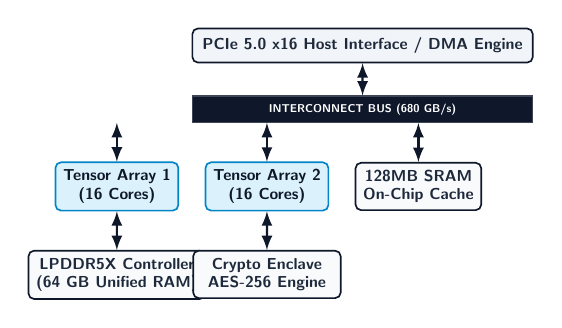
\begin{tikzpicture}[
    scale=0.82, every node/.style={transform shape},
    node distance=6mm and 8mm,
    block/.style={rectangle, draw=Primary, fill=BgLight, rounded corners=2pt, minimum height=1.5em, minimum width=4.2em, align=center, font=\scriptsize\bfseries\color{TextDark}, line width=0.6pt},
    core/.style={rectangle, draw=AccentDark, fill=Accent!15, rounded corners=2pt, minimum height=1.5em, minimum width=4.2em, align=center, font=\scriptsize\bfseries\color{Primary}, line width=0.6pt},
    bus/.style={rectangle, draw=Primary!80, fill=Primary, minimum height=0.4em, minimum width=15em, align=center, font=\tiny\bfseries\color{white}},
    arrow/.style={latex-latex, thick, Primary}
  ]
    % Host Interface
    \node (pcie) [block, minimum width=15em, fill=CardBg] {PCIe 5.0 x16 Host Interface / DMA Engine};

    % Central Bus
    \node (bus1) [bus, below=5mm of pcie] {INTERCONNECT BUS (680 GB/s)};

    % Core Modules
    \node (t1) [core, below left=6mm and 2mm of bus1] {Tensor Array 1\\(16 Cores)};
    \node (t2) [core, right=4mm of t1] {Tensor Array 2\\(16 Cores)};
    \node (sram) [block, right=4mm of t2] {128MB SRAM\\On-Chip Cache};

    % Lower Modules
    \node (memctrl) [block, below=6mm of t1, minimum width=6.5em] {LPDDR5X Controller\\(64 GB Unified RAM)};
    \node (sec) [block, below=6mm of t2, minimum width=6.5em] {Crypto Enclave\\AES-256 Engine};

    % Connections
    \draw [arrow] (pcie) -- (bus1);
    \draw [arrow] (bus1.south -| t1.north) -- (t1.north);
    \draw [arrow] (bus1.south -| t2.north) -- (t2.north);
    \draw [arrow] (bus1.south -| sram.north) -- (sram.north);
    \draw [arrow] (t1) -- (memctrl);
    \draw [arrow] (t2) -- (sec);
  \end{tikzpicture}
  \end{center}

\end{minipage}%
\hfill
\begin{minipage}[t]{0.485\textwidth}

  % --- TECHNICAL SPECIFICATIONS TABLE ---
  \sectionheading{\faSlidersH}{Technical Specifications}

  \small
  \begin{tabularx}{\textwidth}{>{\bfseries\color{TextDark}}l X}
    \toprule
    \rowcolor{Primary!10}
    \multicolumn{2}{l}{\textcolor{Primary}{\bfseries COMPUTE \& PERFORMANCE}} \\
    \midrule
    Peak Performance & 750 INT8 TOPS / 375 BF16 TFLOPS \\{}
    Tensor Execution & 32 Matrix Pipeline Units \\{}
    On-Chip Cache & 128 MB High-Bandwidth SRAM \\{}
    Precision Support & FP16, BF16, INT8, INT4, TF32 \\
    \midrule
    \rowcolor{Primary!10}
    \multicolumn{2}{l}{\textcolor{Primary}{\bfseries MEMORY \& INTERFACE}} \\
    \midrule
    Memory Capacity & 64 GB Unified LPDDR5X \\{}
    Memory Bandwidth & 680 GB/s (256-bit bus) \\{}
    Host Interface & PCIe 5.0 x16 (Up to 64 GB/s) \\{}
    Chip-to-Chip & Dual UltraLink 100 Gbps ports \\
    \midrule
    \rowcolor{Primary!10}
    \multicolumn{2}{l}{\textcolor{Primary}{\bfseries ELECTRICAL \& THERMAL}} \\
    \midrule
    Power Consumption & 75 W Active Peak / 8 W Idle \\{}
    Form Factor & Standard PCIe Single-Slot FHHL \\{}
    Thermal Solution & Passive Heatsink / Active Fan Option \\{}
    Operating Temp & $-40^\circ\text{C}$ to $+85^\circ\text{C}$ (Industrial) \\
    \midrule
    \rowcolor{Primary!10}
    \multicolumn{2}{l}{\textcolor{Primary}{\bfseries SOFTWARE \& COMPLIANCE}} \\
    \midrule
    Software Stack & Synapse Neural Studio v4.2 \\{}
    Frameworks & PyTorch, TensorFlow, ONNX, C++ \\{}
    Certifications & CE, FCC Class A, RoHS, ISO 9001 \\
    \bottomrule
  \end{tabularx}

  \vspace{4pt}

  % --- APPLICATIONS ---
  \sectionheading{\faMicrochip}{Target Workloads \& Applications}
  \vspace{2pt}
  \begin{tabularx}{\textwidth}{@{}l X@{}}
    \textcolor{AccentDark}{\faEye} \textbf{Vision Analytics:} & Real-time 4K multi-stream object tracking and video segmentation.\\{}
    \textcolor{AccentDark}{\faCommentDots} \textbf{LLM Edge Serving:} & Low-latency token generation for 7B--13B parameter models.\\{}
    \textcolor{AccentDark}{\faLock} \textbf{Automotive \& Robotics:} & High-reliability sensor fusion for autonomous vehicle systems.
  \end{tabularx}

\end{minipage}

\vspace{6pt}

% ==================== ORDERING & FOOTER ====================
\begin{tcolorbox}[
  colback=BgLight,
  colframe=Primary,
  arc=3pt,
  left=8pt,right=8pt,top=6pt,bottom=6pt,
  boxrule=0.8pt
]
  \begin{minipage}[t]{0.52\textwidth}
    \textcolor{Primary}{\bfseries\small ORDERING INFORMATION}\\[3pt]
    \tiny
    \begin{tabular}{@{}lll@{}}
      \textbf{Part Number} & \textbf{Memory} & \textbf{Grade \& Thermal} \\
      \hline
      \texttt{SYN-X9-64G-I} & 64 GB LPDDR5X & Industrial ($-40^\circ\text{C}$ to $+85^\circ\text{C}$), Passive \\
      \texttt{SYN-X9-64G-C} & 64 GB LPDDR5X & Commercial ($0^\circ\text{C}$ to $+70^\circ\text{C}$), Active Fan \\
      \texttt{SYN-X9-32G-C} & 32 GB LPDDR5X & Commercial ($0^\circ\text{C}$ to $+70^\circ\text{C}$), Active Fan \\
    \end{tabular}
  \end{minipage}%
  \hfill
  \begin{minipage}[t]{0.44\textwidth}
    \raggedleft
    \textcolor{Primary}{\bfseries\small SYNAPSE TECHNOLOGIES INC.}\\[2pt]
    \textcolor{TextMuted}{\tiny 450 Innovation Parkway, Suite 800, Tech District}\\[1pt]
    \textcolor{TextMuted}{\tiny\faEnvelope\ \texttt{sales@synapse-tech.example} \quad \faGlobe\ \texttt{www.synapse-tech.example}}\\[1pt]
    \textcolor{TextMuted}{\tiny\faPhone\ +1 (800) 555-0199 \quad \copyright\ 2026 Synapse Technologies. All rights reserved.}
  \end{minipage}
\end{tcolorbox}

\end{document}
